%% Figure from MATH 556 notes, section 45 (Lecture 19). ADDED (not from lecture).
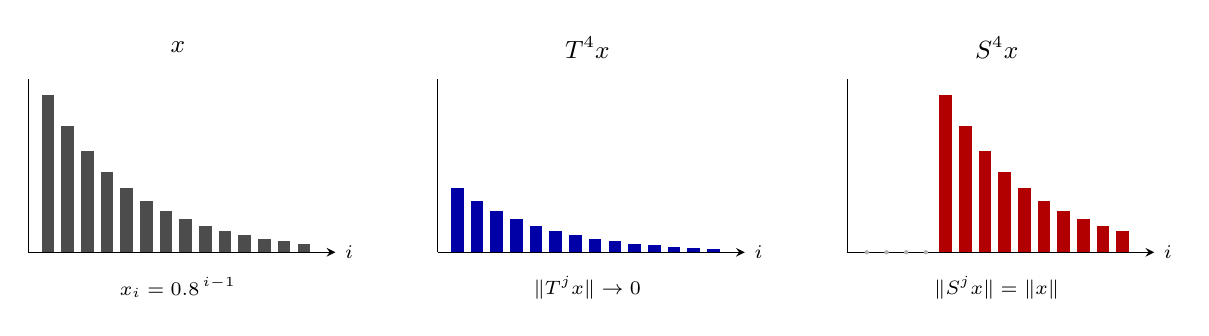
\begin{tikzpicture}[>=stealth]
  \begin{scope}
    \draw[->] (0,0) -- (3.9,0) node[right, font=\scriptsize] {$i$};
    \draw (0,0) -- (0,2.2);
    \foreach \i in {1,...,14} \fill[black!70] ({0.25*\i-0.08},0) rectangle ({0.25*\i+0.08},{2*pow(0.8,\i-1)});
    \node[font=\small] at (1.9,2.6) {$x$};
    \node[font=\scriptsize] at (1.9,-0.45) {$x_i = 0.8^{\,i-1}$};
  \end{scope}
  \begin{scope}[xshift=5.2cm]
    \draw[->] (0,0) -- (3.9,0) node[right, font=\scriptsize] {$i$};
    \draw (0,0) -- (0,2.2);
    \foreach \i in {1,...,14} \fill[blue!65!black] ({0.25*\i-0.08},0) rectangle ({0.25*\i+0.08},{2*pow(0.8,\i+3)});
    \node[font=\small] at (1.9,2.6) {$T^4 x$};
    \node[font=\scriptsize] at (1.9,-0.45) {$\|T^j x\| \to 0$};
  \end{scope}
  \begin{scope}[xshift=10.4cm]
    \draw[->] (0,0) -- (3.9,0) node[right, font=\scriptsize] {$i$};
    \draw (0,0) -- (0,2.2);
    \foreach \i in {1,...,4} \fill[gray!60] ({0.25*\i},0) circle (0.8pt);
    \foreach \i in {5,...,14} \fill[red!70!black] ({0.25*\i-0.08},0) rectangle ({0.25*\i+0.08},{2*pow(0.8,\i-5)});
    \node[font=\small] at (1.9,2.6) {$S^4 x$};
    \node[font=\scriptsize] at (1.9,-0.45) {$\|S^j x\| = \|x\|$};
  \end{scope}
\end{tikzpicture}
